\documentclass{article}
\usepackage{float}
\usepackage{tikz}
\usetikzlibrary{decorations.pathreplacing}
\usetikzlibrary{positioning}
\title{BSDCONV}
\date{}
\begin{document}
	\maketitle
	\tableofcontents
	\section{Syntax}
		\subsection{Phases \& Cascade}
			\begin{figure}[H]
				\centering
				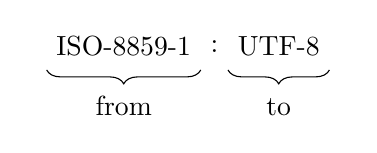
\begin{tikzpicture}[auto,node distance=0,on grid=false]

				    % Place nodes
				    \node (d0) {};
				    \node [right=of d0](from) {ISO-8859-1};
				    \node [right=of from](d1) {:};
				    \node [right=of d1] (to) {UTF-8};
				    \node [right=of to] (d2) {};
					
					\draw [decorate,decoration={brace,amplitude=5pt,raise=3mm, mirror}]
(d0)--(d1)  node  [black,midway,yshift=-1cm] { from };
				
					\draw [decorate,decoration={brace,amplitude=5pt,raise=3mm, mirror}]
(d1) -- (d2)  node [black,midway,yshift=-1cm] { to };
				
				\end{tikzpicture}
				\caption{Basic two phases conversion}
			\end{figure}
			
			\begin{figure}[H]
				\centering
				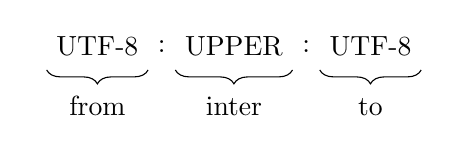
\begin{tikzpicture}[auto,node distance=0,on grid=false]			
				    % Place nodes
				    \node (d0) {};
				    \node [right=of d0](from) {UTF-8};
				    \node [right=of from](d1) {:};
				    \node [right=of d1] (inter) {UPPER};
				    \node [right=of inter](d2) {:};
				    \node [right=of d2] (to) {UTF-8};
				    \node [right=of to] (d3) {};			
					
					\draw [decorate,decoration={brace,amplitude=5pt,raise=3mm, mirror}]
	(d0) -- (d1) node [black,midway,yshift=-1cm] { from };
					
					\draw [decorate,decoration={brace,amplitude=5pt,raise=3mm, mirror}]
	(d1) -- (d2) node [black,midway,yshift=-1cm] { inter };
					
					\draw [decorate,decoration={brace,amplitude=5pt,raise=3mm, mirror}]
	(d2) -- (d3) node [black,midway,yshift=-1cm] { to };
				\end{tikzpicture}
				\caption{Conversion with inter-mapping phase}
			\end{figure}
			
			\begin{figure}[H]
				\centering
				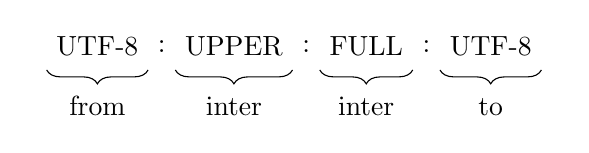
\begin{tikzpicture}[auto,node distance=0,on grid=false]
				    % Place nodes
				    \node (d0) {};
				    \node [right=of d0](from) {UTF-8};
				    \node [right=of from](d1) {:};
				    \node [right=of d1] (inter) {UPPER};
				    \node [right=of inter](d2) {:};
				    \node [right=of d2] (inter2) {FULL};
				    \node [right=of inter2](d3) {:};
				    \node [right=of d3] (to) {UTF-8};
				    \node [right=of to] (d4) {};			
					
					\draw [decorate,decoration={brace,amplitude=5pt,raise=3mm, mirror}]
	(d0) -- (d1) node [black,midway,yshift=-1cm] { from };
					
					\draw [decorate,decoration={brace,amplitude=5pt,raise=3mm, mirror}]
	(d1) -- (d2) node [black,midway,yshift=-1cm] { inter };
					
					\draw [decorate,decoration={brace,amplitude=5pt,raise=3mm, mirror}]
	(d2) -- (d3) node [black,midway,yshift=-1cm] { inter };
					
					\draw [decorate,decoration={brace,amplitude=5pt,raise=3mm, mirror}]
	(d3) -- (d4) node [black,midway,yshift=-1cm] { to };
				
				\end{tikzpicture}
				\caption{Conversion with multiple inter-mapping phases}
			\end{figure}
	
			\begin{figure}[H]
				\centering
				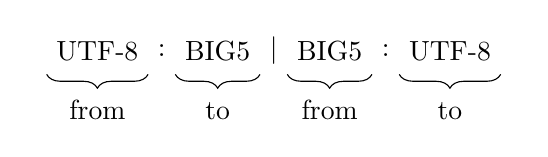
\begin{tikzpicture}[auto,node distance=0,on grid=false]
				    % Place nodes
				    \node (d0) {};
				    \node [right=of d0] (from) {UTF-8};
				    \node [right=of from] (d1) {:};
				    \node [right=of d1] (to) {BIG5};
				    \node [right=of to] (d2) {$|$};
				    \node [right=of d2] (from2) {BIG5};
				    \node [right=of from2](d3) {:};
				    \node [right=of d3](to2) {UTF-8};
				    \node [right=of to2] (d4) {};
					
					\draw [decorate,decoration={brace,amplitude=5pt,raise=3mm, mirror}] (d0) -- (d1) node [black,midway,yshift=-1cm] { from };
				
					\draw [decorate,decoration={brace,amplitude=5pt,raise=3mm, mirror}] (d1) -- (d2) node [black,midway,yshift=-1cm] { to };

					\draw [decorate,decoration={brace,amplitude=5pt,raise=3mm, mirror}] (d2) -- (d3) node [black,midway,yshift=-1cm] { from };

					\draw [decorate,decoration={brace,amplitude=5pt,raise=3mm, mirror}] (d3) -- (d4) node [black,midway,yshift=-1cm] { to };
				
				\end{tikzpicture}
				\caption{Cascaded conversions}
			\end{figure}
		
		\subsection{Codecs \& Fallback}
			\begin{figure}[H]
				\centering
				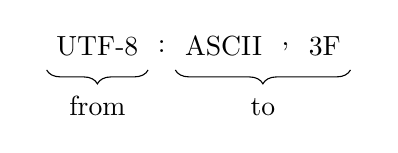
\begin{tikzpicture}[auto,node distance=0,on grid=false]
				    % Place nodes
				    \node (d0) {};
				    \node [right=of d0] (from) {UTF-8};
				    \node [right=of from] (d1) {:};
				    \node [right=of d1] (to) {ASCII};
				    \node [right=of to] (d2) {,};
				    \node [right=of d2] (from2) {3F};
				    \node [right=of from2] (d3) {};
					
					\draw [decorate,decoration={brace,amplitude=5pt,raise=3mm, mirror}] (d0) -- (d1) node [black,midway,yshift=-1cm] { from };
				
					\draw [decorate,decoration={brace,amplitude=5pt,raise=3mm, mirror}] (d1) -- (d3) node [black,midway,yshift=-1cm] { to };
				
				\end{tikzpicture}
				\caption{Fallback codec}
			\end{figure}
			
		\subsection{Codec argument}
			\begin{figure}[H]	
				\centering
				\begin{tikzpicture}[auto,node distance=0,on grid=false]
				    % Place nodes
				    \node (d0) {};
				    \node [right=of d0] (from) {UTF-8};
				    \node [right=of from] (d1) {:};
				    \node [right=of d1] (to) {ASCII};
				    \node [right=of to] (d2) {,};
				    \node [right=of d2] (to2) {ANY\#3F};
				    \node [right=of from2] (d3) {};
				
				\end{tikzpicture}
				\caption{Passing argument to codec}
			\end{figure}
			
			\begin{figure}[H]
				\centering
				
\begin{tikzpicture}[auto,node distance=0,on grid=false]
				    % Place nodes
				    \node (d0) {};
				    \node [right=of d0](from) {UTF-8};
				    \node [right=of from](d1) {:};
				    \node [right=of d1] (to) {ASCII};
				    \node [right=of to] (d2) {,};
				    \node [right=of d2] (to2) {ESCAPE\#PREFIX=2575};
				    \node [right=of to2] (d3) {};
				
				\end{tikzpicture}
				\caption{Passing argument to codec in key=value form}
			\end{figure}
			
			\begin{figure}[H]
				\centering
				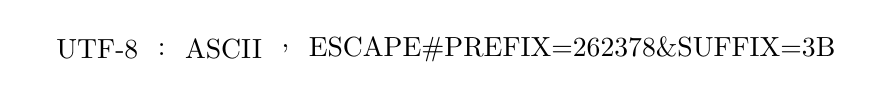
\begin{tikzpicture}[auto,node distance=0,on grid=false]
				    % Place nodes
				    \node (d0) {};
				    \node [right=of d0](from) {UTF-8};
				    \node [right=of from](d1) {:};
				    \node [right=of d1] (to) {ASCII};
				    \node [right=of to] (d2) {,};
				    \node [right=of d2] (to2) {ESCAPE\#PREFIX=262378\&SUFFIX=3B};
				    \node [right=of to2] (d3) {};
				
				\end{tikzpicture}
				\caption{Passing multiple arguments to codec}
			\end{figure}

	\section{Type \& Flag}
		\subsection{Type}
			\paragraph{}
				\begin{table}[H]
					\centering
					\begin{tabular}{|c | l | c | c|}
						\hline
						ID & Description & Provider(from) & Consumer(to)\\
						\hline
						00 & Bsdconv special characters & BSDCONV\_KEYWORD & BSDCONV\_KEYWORD\\
						01 & Unicode & Most decoder & Most encoder\\
						02 & CNS11643 & CNS11643 & CNS11643\\
						03 & Byte & BYTE; ESCAPE & BYTE; ESCAPE\#MODE=\{8,16\}\\
						04 & Chinese components & inter/ZH\_DECOMP & inter/ZH\_COMP\\
						1B & ANSI control sequence & ANSI-CONTROL & -\\
						\hline
					\end{tabular}
					\caption{Types and its provider/consumer (just to name a few)}
				\end{table}
			\paragraph{}
				As for the intersection of CNS11643 and Unicode, from/CNS11643 does conversion to unicode type if possible. Vice versa, to/CNS11643 does conversion from unicode type if possible.
			\paragraph{}
				
\end{document}
